\chapter{CYTO AI}

CYTO AI is the first fully web-based image labeling and classifying tool publicly available. Based on the JavaScript frameworks React and TensorFlow.js,
all advantages of modern machine learning and labeling
technology could be employed in a zero installation effort,
completely platform independent, and fully browser based
solution.

This rich client application does not require the upload of
any data to a server. This helps both, privacy concerns as well as performance. The following sections shall explain how CYTO AI works and which techniques and architectures were used to build it.

\begin{figure}[H]
	\centering
	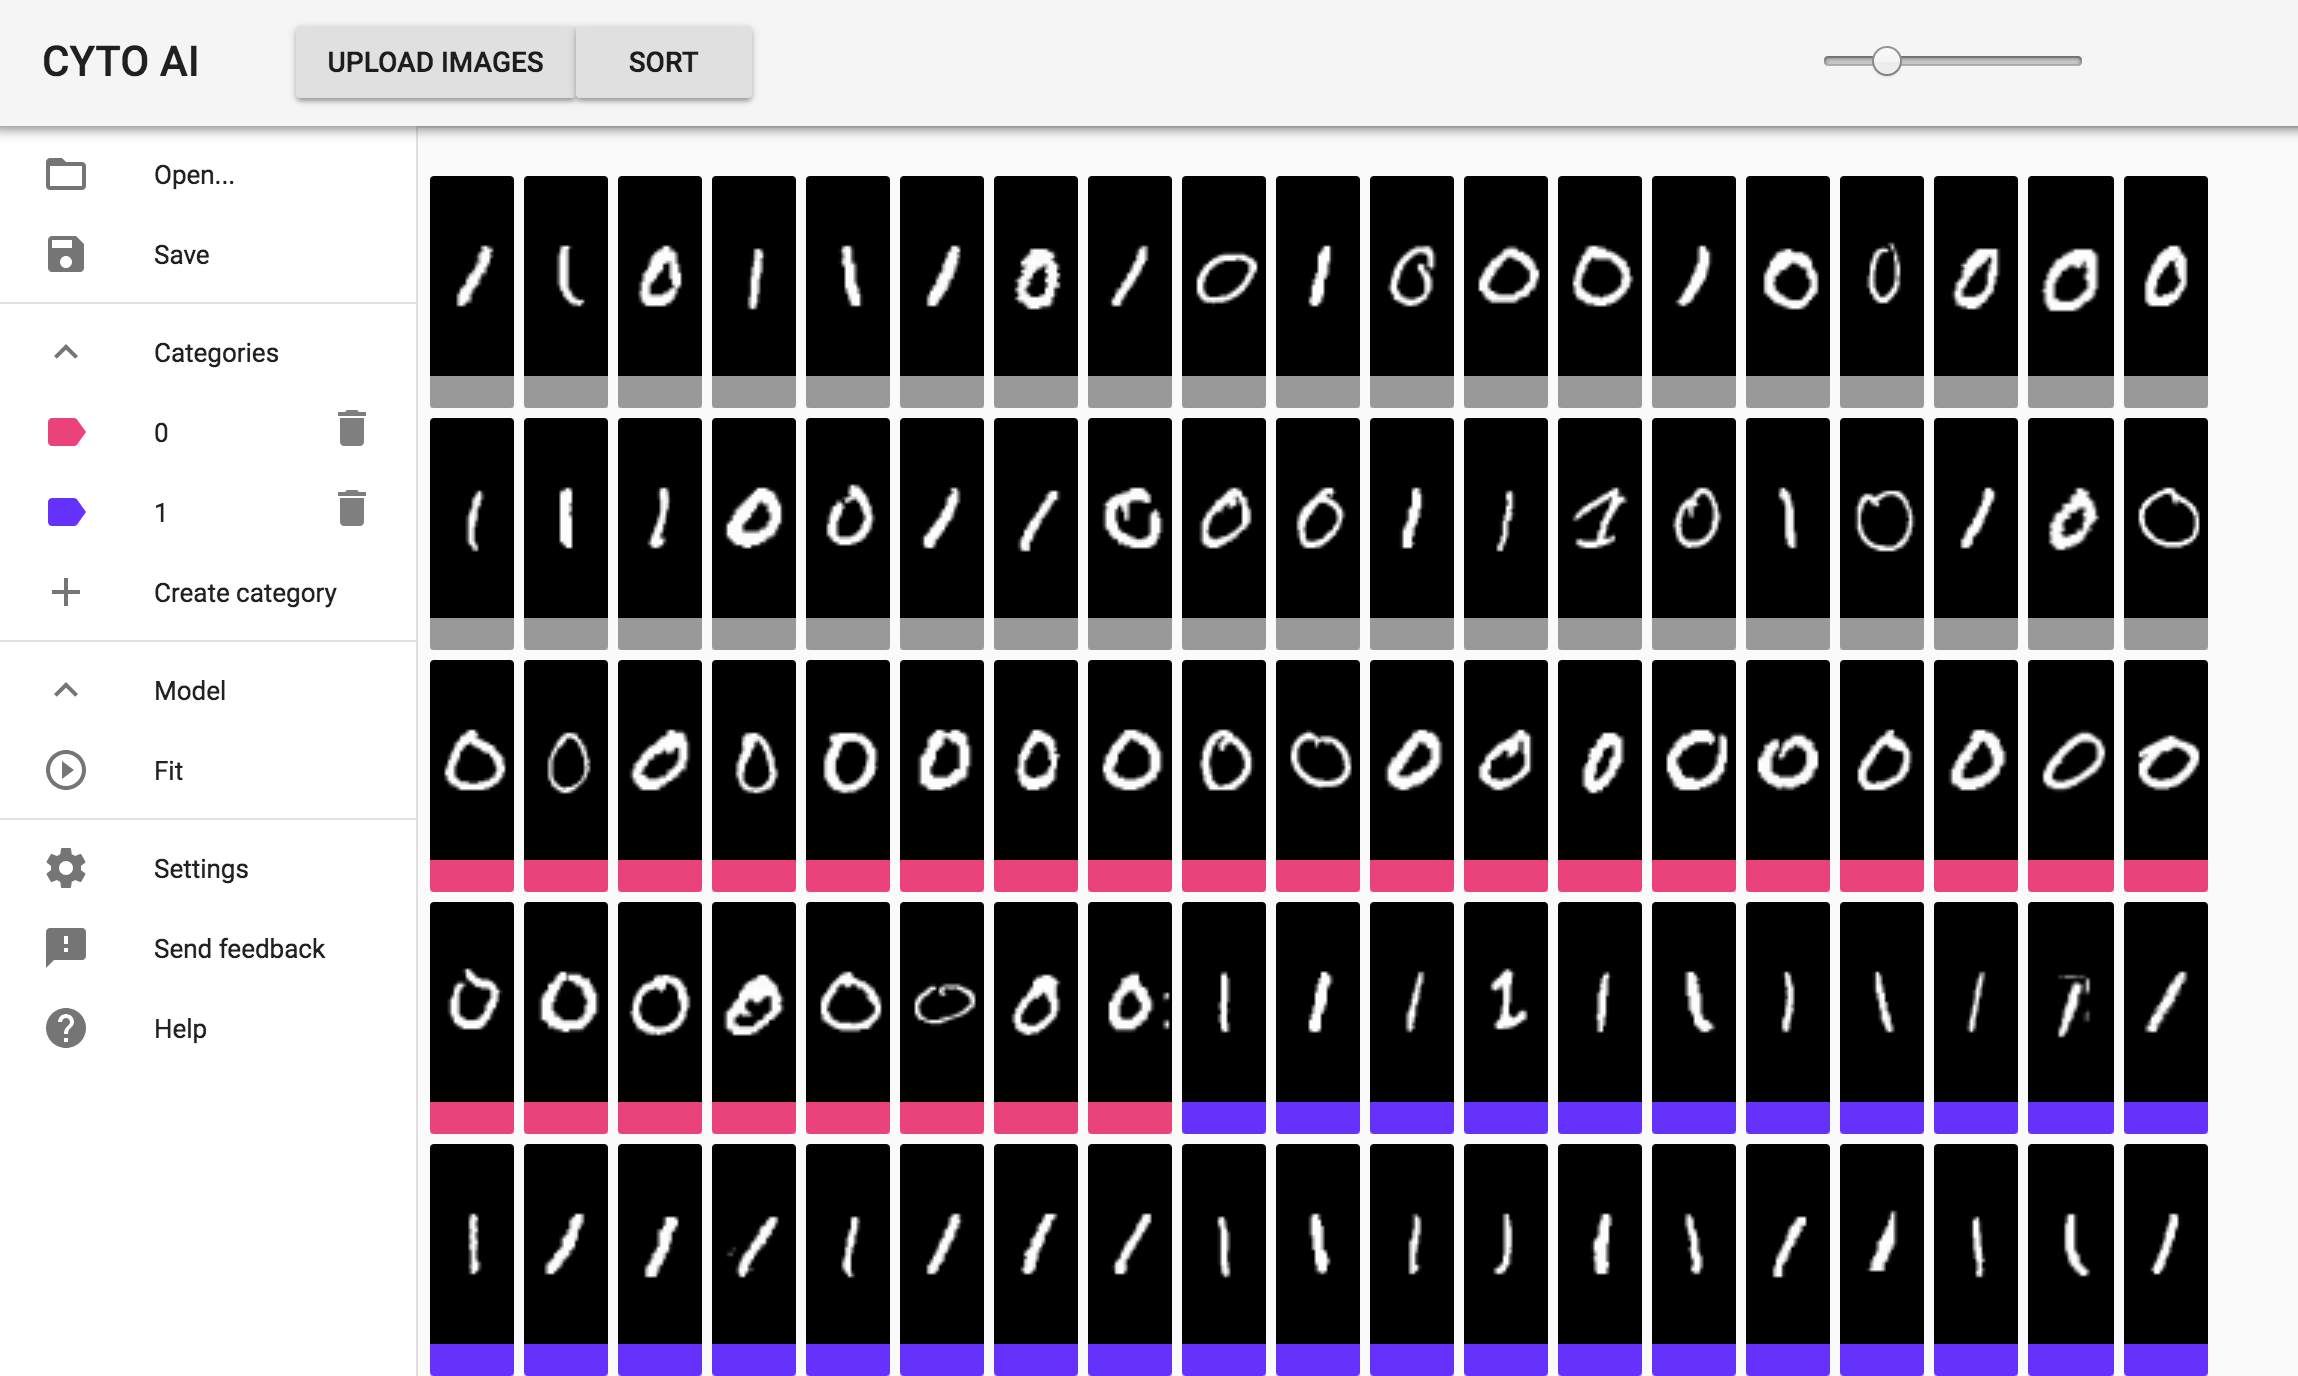
\includegraphics[width=0.8\linewidth]{bilder/cyto/cyto.png}
	\caption{CYTO AI}
	\label{fig:COMPONENT}
\end{figure}


\subsection{Workflow overview}

The workflow starts with the creation of categories. Each image to be classified will have to be assigned to a category.

\begin{figure}[H]
	\centering
	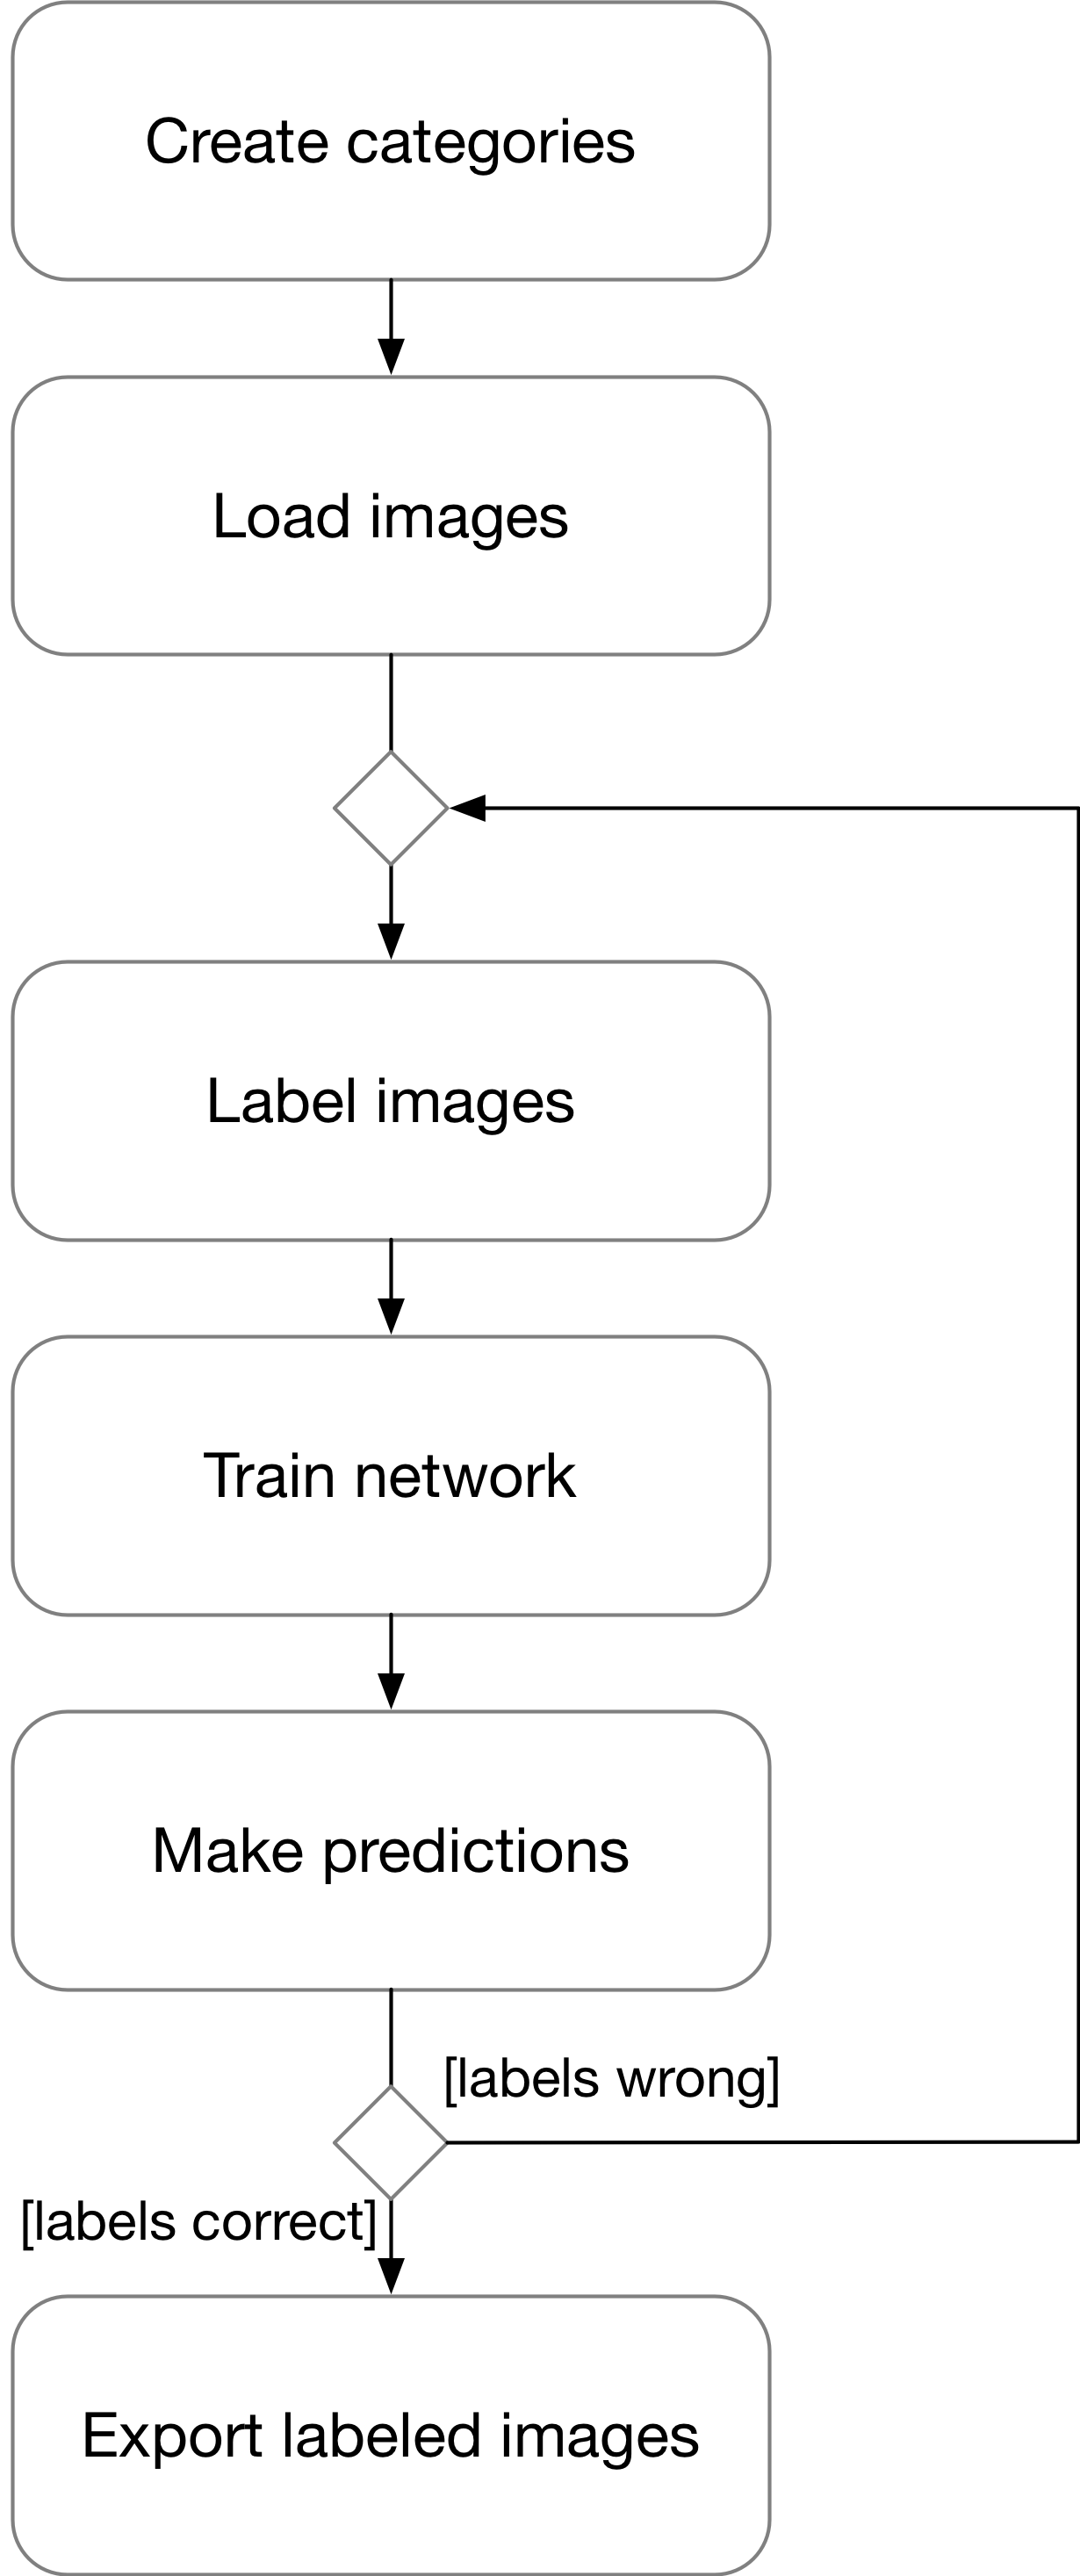
\includegraphics[scale=0.6]{bilder/cyto/Ablaufdiagramm.png}
	\caption{Workflow}
	\label{fig:Workflow}
\end{figure}

Now the images need to be made available to the application.
They are being uploaded to the local browser cache.
It is possible to select entire folders which will result in being all images in that folder and their sub-folders being uploaded.

Once all images have been uploaded a knowledgeable user has
to classify them by dragging them to the respective category field.

After sufficient samples haves been categorized the network
can be trained. Depending the amount of images this can take more or less time. The training results in a trained network.
Which now can be used to classify the previously
unclassified images. This machine labeling needs to
be controlled by a knowledgeable user
and erroneous annotations have to be manually corrected.

Thereafter the network is trained again. This procedure is 
repeated until the labeling error rate by the trained
network is satisfactory.

Now the labeled images can be exported and used by others
to train their networks. In future it will be possible to
export the network parameters so that a complete trained
can be shared with others.


\section{Working with CYIO AI}

\subsection{Creating categories}
To add a category click on button A in figure \ref{fig:Category}. To delete a category click on the corresponding trash can symbol. 
It is not possible right now to directly change a category.
For changing a category you need to delete the old one and
create a new one.

\begin{figure}[H]
	\centering
	\includegraphics[scale=0.8]{bilder/cyto/categories.png}
	\caption{Create a ctagory}
	\label{fig:Category}
\end{figure}

\subsection{Uploading images}
In order to upload images click on button A in figure \ref{fig:ImageUpload}.
In Chrome and Firefox it is possible to select entire folders.
All images have to be in the portable network graphics format (PNG).

\begin{figure}[H]
	\centering
	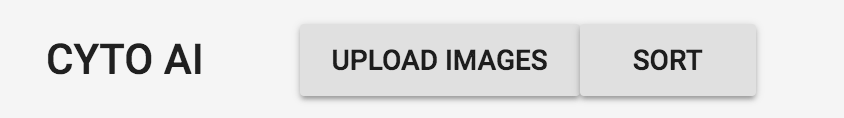
\includegraphics[scale=0.6]{bilder/cyto/UploadImages.png}
	\caption{Image upload}
	\label{fig:ImageUpload}
\end{figure}


\subsection{Labeling images}

There are two ways to annoate an image.

\begin{itemize}
	\item Drag an image and drop it on the desired category.
	\item Select an image and use the keyboard for annotation
\end{itemize}
 First it is possible
to 
A different way is to click on one picture in order to
select it an then use the keyboard to annotate the image.
Following keys are supported to annotate an image:

\begin{itemize}
	\item \keystroke{ 1 } \keystroke{2} \keystroke{3} \keystroke{4} \keystroke{5} \keystroke{6} \keystroke{7}
	\keystroke{8} \keystroke{9} \keystroke{0} where \keystroke{1} is the first category in list.
	\item \keystroke{$\Leftarrow$} backslash to delete a given category
\end{itemize}

Further it is possible to navigate through all images with the arrow keys \keystroke{$\Uparrow$} to go up in row and 
\keystroke{$\Downarrow$} to go down in row. Further \keystroke{$\Rightarrow$} to go right in column and \keystroke{$\Leftarrow$} to go left in column.


\subsection{Classifying images}

For classifying the fit button needs to be clicked.
The neural network will be trained and all unlabeled
images will be categorized.

\begin{figure}[H]
	\centering
	
\includegraphics[scale=0.8]{bilder/cyto/Fit.png}
	\caption{Classify images}
	\label{fig:Clssify}
\end{figure}

By that all unlabeled images will be given a category and a number will be shown under the image. This number is the probability an image belongs to the given category.

\subsection{Exporting}

To save all labels and categories and settings the button save can be pressed. To import again the "open" button can be used. The files will be exported in a JSON format.

\begin{figure}[H]
	\centering
	
\includegraphics[scale=0.8]{bilder/cyto/OpenSave.png}
	\caption{Export and import labels}
	\label{fig:ExportImport}
\end{figure}

\subsection{Filtering and sorting}
 
Also it is possible to blend out certain categories by
clicking on the category, clicking another time will blend
in the category. That gives the possibility to only show
certain categories or to only show unlabeled images.
If all categories are blended out it is still possible to
annotate, newly labeled image will stay visible.
 
\begin{figure}[H]
 	\centering
 	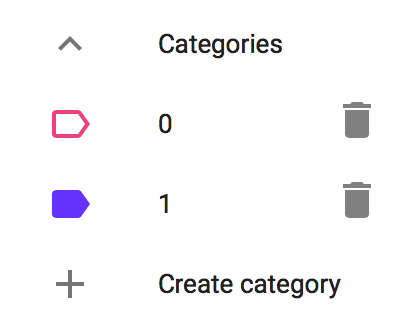
\includegraphics[scale=0.8]{bilder/cyto/BlendedOut.png}
 	\caption{Blending out images with category}
 	\label{fig:BlendingOut}
\end{figure}
  
If pictures were labeled it makes sense to sort them, this
is possible by clicking the sort button. This improves the
overview and makes reviewing labels easier. Uncategorized
images will always appear at the top.
 
Another feature that improves the overview is the slider. The slider makes it possible to adjust the number of displayed images per row. 

\begin{figure}[H]
	\centering
	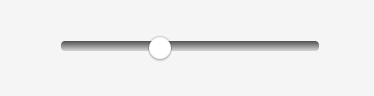
\includegraphics[scale=0.8]{bilder/cyto/Slider.png}
	\caption{Slider adjusts number of pictures displayed per row}
	\label{fig:Slider}
\end{figure}

\section{IDE setup}
Following IDE setup was chosen to develop CYTO AI.
Visual Studio Code was introduced in 2016. It porovides integrated GIT support as well as easy debugging, syntax highlighting and an intelligent code completion.
We used the integrated terminal and installed a JavaScript syntax checker called ESLint, further we are using a code formatter called Prettier. 

\begin{figure}[H]
	\centering
	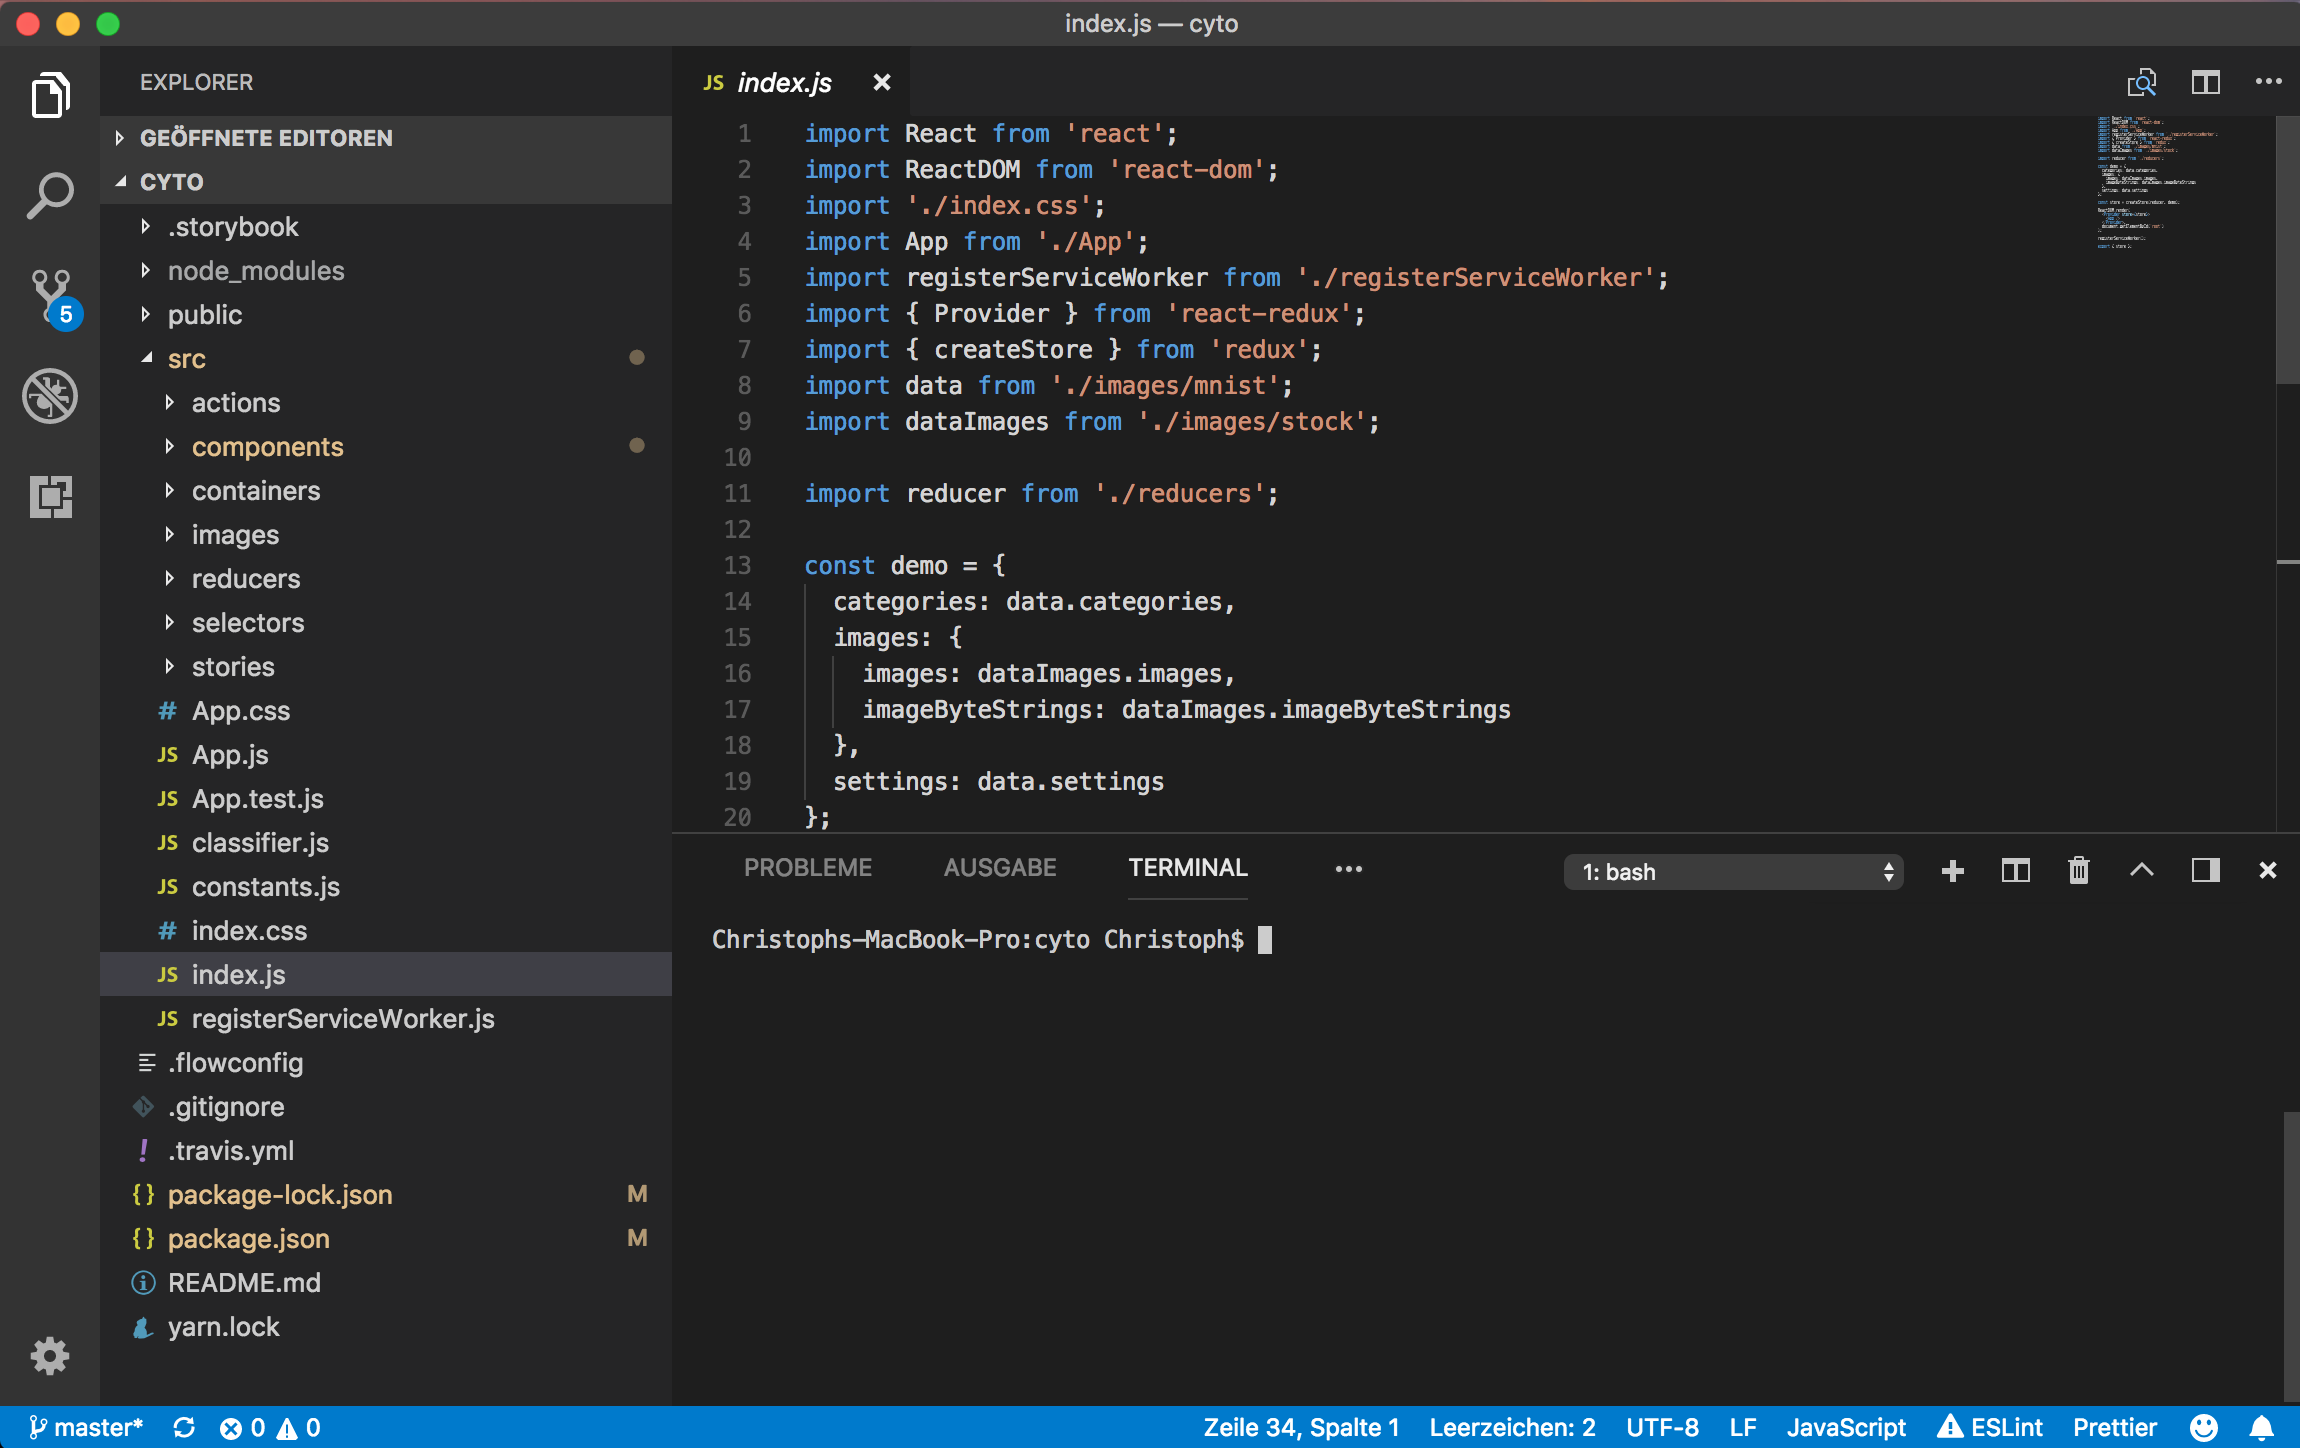
\includegraphics[width=\linewidth]{bilder/cyto/IDE.png}
	\caption{IDE setup}
	\label{fig:IDE}
\end{figure}

\begin{figure}[H]
	\centering
	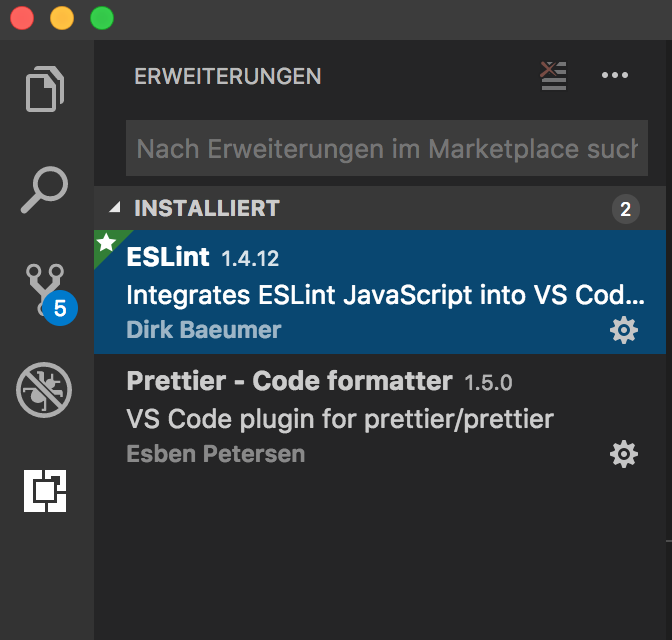
\includegraphics[scale=0.5]{bilder/cyto/LINT.png}
	\caption{Used extensions}
	\label{fig:Extensions}
\end{figure}

\section{Package management}
For managing dependencies and necessary frameworks npm is used. 

Packages can be installed via:

	\texttt{npm i ---save string-hash}

and be used by importing it:

	\texttt{import hash from 'string-hash'} \\
	\texttt{let identifier = hash(e.target.result)}

all used packaged are going to be saved in the node\_modules
folder. Further all used packaged will be written inside the
package.json file.


\section{The edit-debug cycle}

Make sure to download and install Node.Js. It can be found under

\texttt{https://nodejs.org/en/download/}

The application needs to be downloaded:

\texttt{git clone https://github.com/cytoai/cyto.git}

Within the application folder following commands are used to
run the app.

After downloading all dependencies need to be installed:

\texttt{npm install}

Then the local Node.js server can be created by:

\texttt{npm start}

To debug within in the browser a plugin React Developer Tools
for Google Chrome was installed. With React Developer Tools
it is possible to inspect rendered components and highlight DOM updates 

\begin{figure}[H]
	\centering
	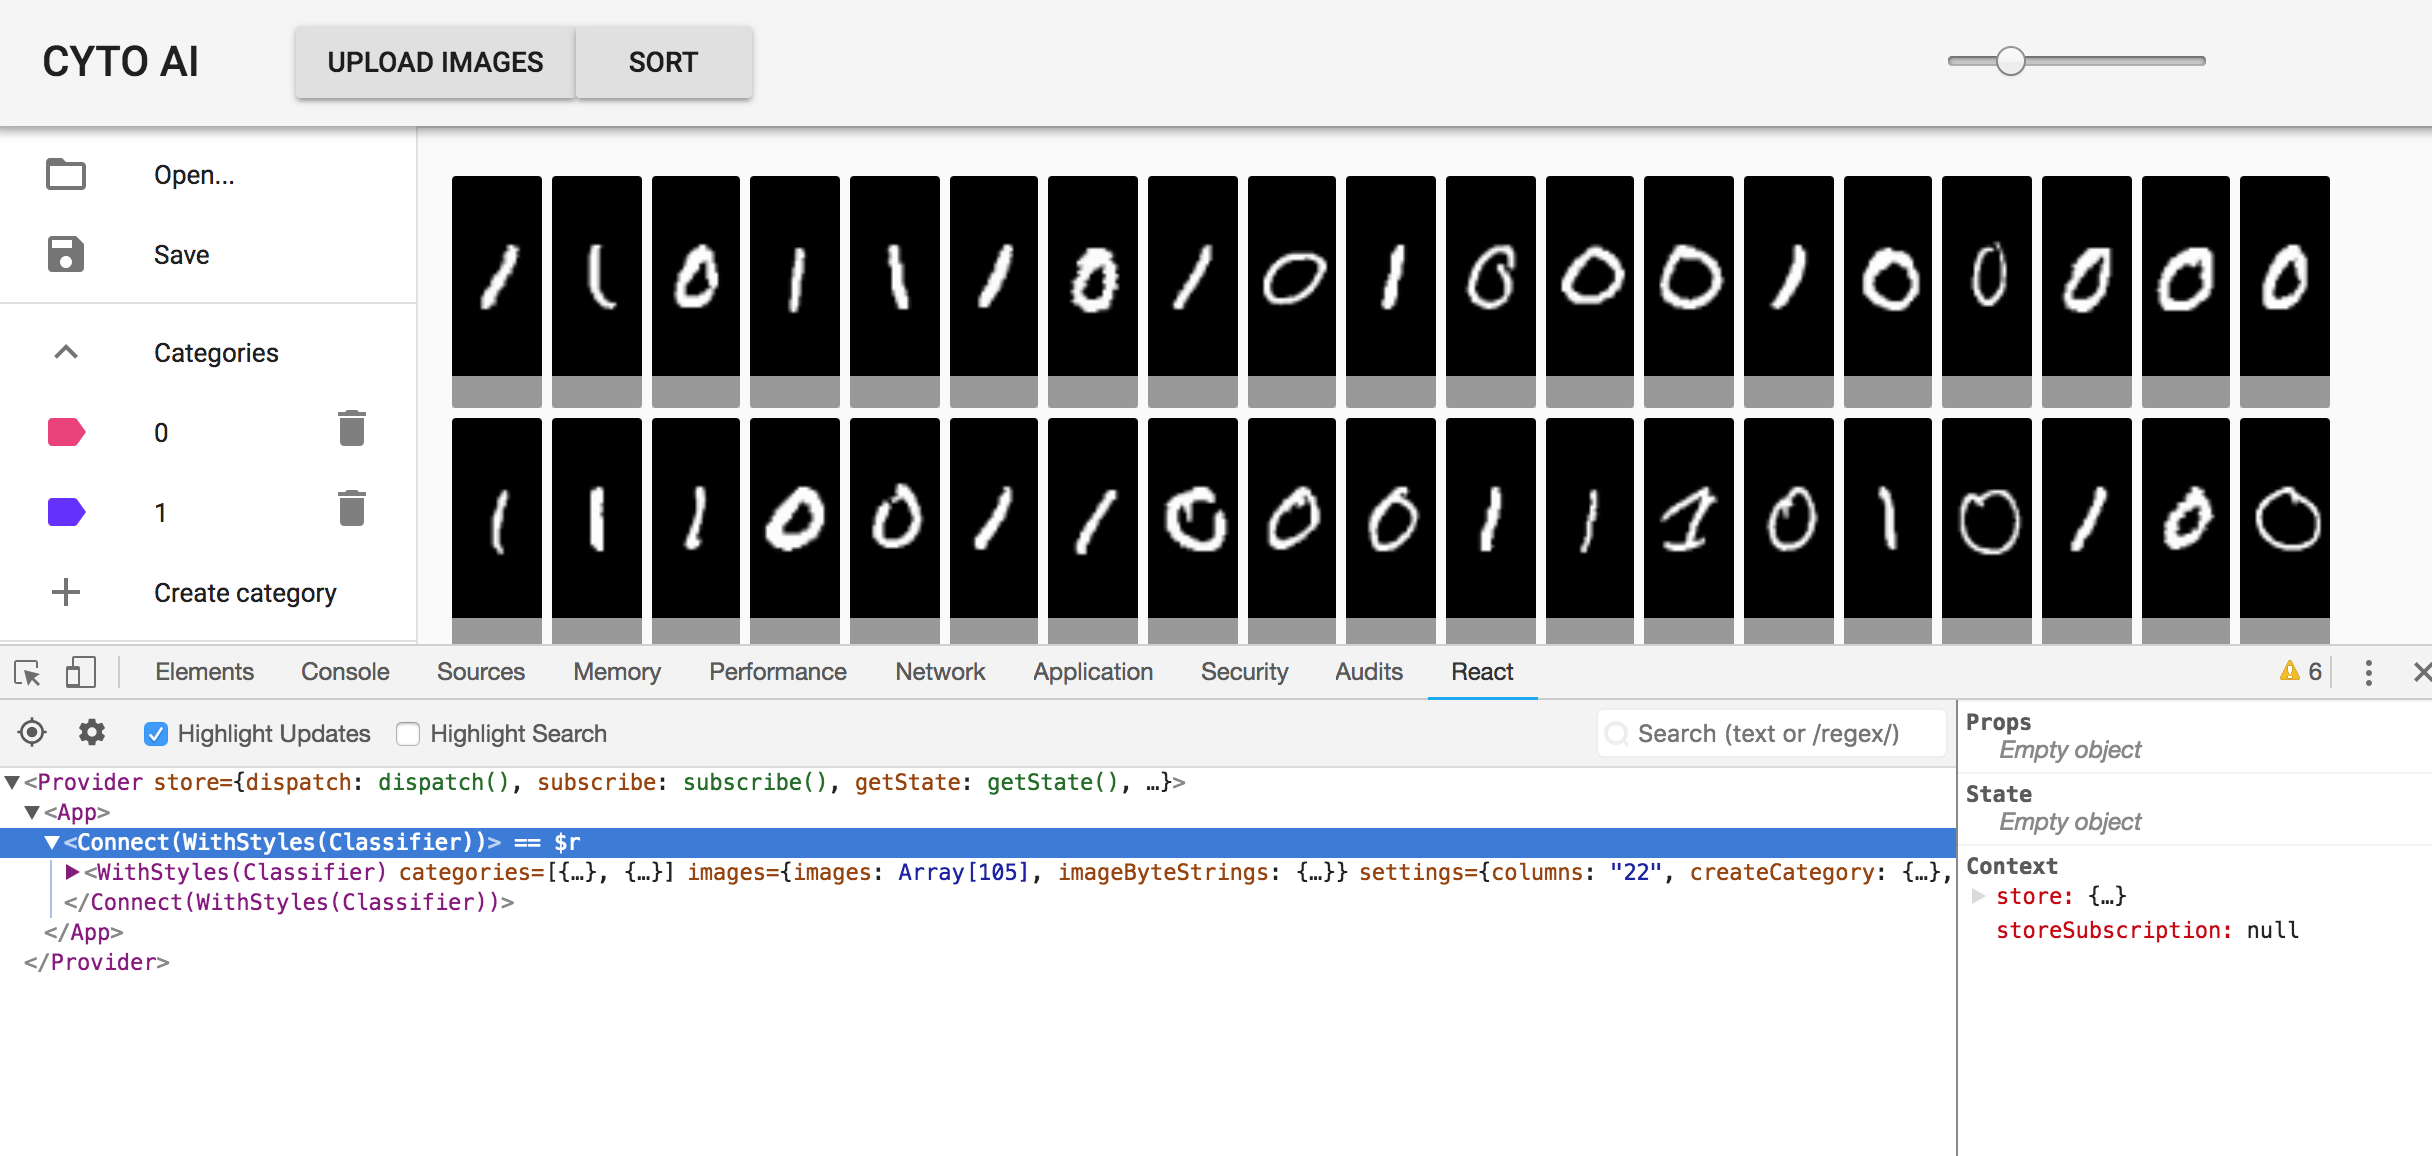
\includegraphics[width=0.9\linewidth]{bilder/cyto/ReactDebug.png}
	\caption{React developer tools}
	\label{fig:Developer Tools}
\end{figure}

The project was set up to reload the browser every time 
the code changes. There is not need to empty the cash or reload the browser manually.


\section{System architecture overview}

To explain the structure of the system an example will be used. A component shall be added to the running application,
by that it shall be clear how the system works.

\subsection{Adding a component}
First a new component "Categories" is created. Categories shall simply show a list of categories. 

\lstinputlisting[caption=Categories component ]{code/cyto/categoryList.js}

The data shall be fetched from a variable categories that is
placed in the Redux store.
In order to fetch this data the component shall be connected to the Redux store so a High-Order Component ConnectedCategories is created.
The connector adds the possibility to access the categories array in the Redux store.

\lstinputlisting[caption=Connector component]{code/cyto/connectedCategory.js}

Further it shall be possible to add another category to the category list, therefore an action is needed that takes the new category name and the category color as a payload.

\lstinputlisting[caption=Actions for changing categories]{code/cyto/actions.js}

A reducer will now be called given and the action will be passed to it.

\lstinputlisting[caption=Reducer for changing categories]{code/cyto/categoryReducer.js}


In short for each added component that needs access to the states a connector needs to be created. Actions and reducers also need to be created to change the state, if not already existing.

The directory structure would now look like this:


\begin{figure}[H]
	\centering
	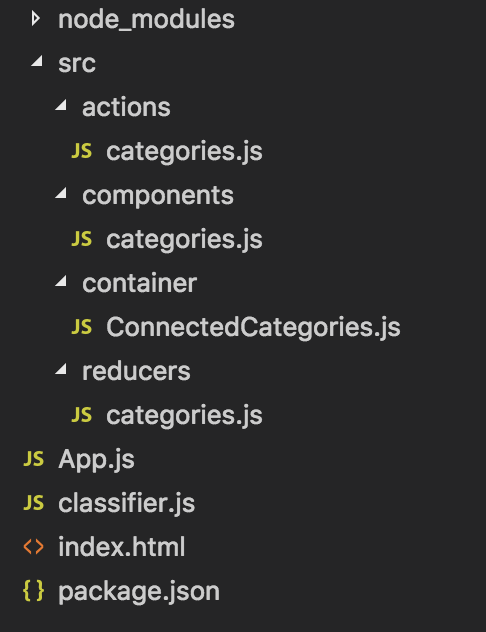
\includegraphics[scale=0.8]{bilder/cyto/SystemArchitecture.png}
	\caption{System architecture ovierview}
	\label{fig:SystemOverview}
\end{figure}


\subsection{The machine learning API}
The machine learning API was built with TensorFlow.js. Every time the "fit" button was clicked an asynchronous API call is made. The calls look like following:

\lstinputlisting[caption=Machine learning API ]{code/cyto/classifier.js}

Where dataset is an instance for handling the data. And imageTags are the HTML . The API is using a CNN Network provided over a Content Delivery Network (CDN).









